

\documentclass [PhD] {uclathes}

\newcommand{\minsum}{Min Sum}

%channel
\newcommand{\y}{\mathbf{y}}
\newcommand{\x}{\mathbf{x}}
\newcommand{\xel}{x}
\newcommand{\xalph}{\mathcal{X}}
\newcommand{\yalph}{\mathcal{Y}}
\newcommand{\noisestd}{\sigma}
\newcommand{\snr}{\mathrm{SNR}}
\newcommand{\dabpmf}{p_{\mathrm{DAB}}}
%message and CRC
\newcommand{\numbits}{k}
\newcommand{\alabelel}{w}
\newcommand{\alabel}{\mathbf{\alabelel}}
\newcommand{\crcquotel}{q}
\newcommand{\crcquot}{\mathbf{\crcquotel}}
\newcommand{\ceq}{\mathbf{G}_{\mathrm{eq}}}
\newcommand{\peq}{\mathbf{P}_{\mathrm{eq}}}
\newcommand{\convc}{\mathbf{G}}
%convolutional encoder
\newcommand{\length}{l}
\newcommand{\uinel}{u}
\newcommand{\uin}{\mathbf{\uinel}}
\newcommand{\convrate}{k}
%Pairwise Error probability
\newcommand{\FER}{\mathrm{FER}}
\newcommand{\pairwiseerrorevent}[1]{\mathbf{e}_{#1}}
%codeword indices; renew when section uses different ones
\newcommand{\corridx}{c}
\newcommand{\erridx}{e}
\newcommand{\errorevent}{\varepsilon_{\mathbf{x}_c}}
\newcommand{\PEE}{e_{\mathbf{x}_c,\mathbf{x}_e}}
\newcommand{\PEP}{P\left(\PEE\right)}
%modified metric
\newcommand{\xc}{\x_{\corridx}}%correct codeword
\newcommand{\xe}{\x_{\erridx}}%incorrect codeword
\newcommand{\uc}{\uin_{\corridx}}%correct codeword
\newcommand{\ue}{\uin_{\erridx}}%incorrect codeword
\newcommand{\yprime}{\mathbf{z}'}
\newcommand{\dplain}{d}
\newcommand{\de}{d_{\mathrm{E}}}
\newcommand{\dnew}{d_{\mathrm{new}}}
\newcommand{\da}{d_{\mathrm{prox}}}
%transfer function
\newcommand{\dfree}{d_{\mathrm{free}}}
\newcommand{\overell}{_{\ell = 1}^\length}
% \newcommand{\errstate}{s}
% \newcommand{\encstate}{r}
% \newcommand{\errstatevec}{\mathbf{\errstate}}
% \newcommand{\encstatevec}{\mathbf{\encstate}}
\newcommand{\eq}{{q}}
\newcommand{\err}{e}
\newcommand{\errstart}{s_\err}
\newcommand{\errend}{s'_\err}
\newcommand{\eqstart}{s_\eq}
\newcommand{\eqend}{s'_\eq}
\newcommand{\erri}{\err_i}
\newcommand{\erro}{\err_o}
\newcommand{\tbcc}{T_{\mathrm{TBCC}}}
\newcommand{\errcnt}{\mathcal{S}_\err}
\newcommand{\eqcnt}{\mathcal{S}_\eq}
%matrices
\newcommand{\bigmat}{\mathbf{G}}
%misc
\newcommand{\reals}{\mathbb{R}}
\newcommand{\pmf}{PMF}
\newcommand{\setedge}{\mathcal{E}}
\newcommand{\setstate}{\mathcal{V}}
\newcommand{\interval}{\mathcal{I}}
\newcommand{\outlen}{n}


\newcommand{\equl}{\Tilde{l}}



%polynomials
\newcommand{\polyvar}{x}
\newcommand{\convpoly}{p(x)}
\newcommand{\uinpoly}{\uinel(\polyvar)}
\newcommand{\uinsplit}{\uin_{\mathrm{split}}(\polyvar)}
\newcommand{\crcquotsplit}{\crcquot_{\mathrm{split}}(\polyvar)}
\newcommand{\alabelsplit}{\alabel_{\mathrm{split}}(\polyvar)}




\newcommand{\soursymsqe}{\mathbf{s}}
\newcommand{\crcinb}{\mathbf{g}}
\newcommand{\crcoutb}{\mathbf{h}}
\newcommand{\crcins}{\mathbf{w}}
\newcommand{\cicous}{\mathbf{u}}
\newcommand{\dmou}{\mathbf{a}}
\newcommand{\chaninsy}{\mathbf{x}}


%%TBCC
\newcommand{\ccinnum}{k_0}
\newcommand{\ccoutnum}{\gamma_0}
\newcommand{\ccoutputset}{\mathcal{O}}
\newcommand{\ccoutputrealize}{o}



                         % personal LaTeX macros
%%-------Linfang Package------
\usepackage{graphicx}
\usepackage{epstopdf}
\usepackage[caption=false,font=footnotesize]{subfig}
\usepackage{cite}
\usepackage{color}
\usepackage{xcolor}
\usepackage[cmex10]{amsmath}
\usepackage{amssymb}
\usepackage{threeparttable}
\usepackage{mathtools}
\usepackage{hyperref}
\usepackage{algpseudocode}
\usepackage{multirow}
\usepackage[T1]{fontenc}
\usepackage[ruled]{algorithm2e}
\usepackage{booktabs}
\usepackage{stfloats}
\usepackage{tensor}
\usepackage{bbm}
\usepackage{multicol}
\usepackage{tikz}
\usepackage{cooltooltips}
\def\cool{\texttt{cool}}
\definecolor{mygreen}{rgb}{0.1,.6,0.1}
\DeclareMathOperator*{\argmax}{argmax} 

%%------Tikz Package------
\usepackage{tikz}
\usetikzlibrary{shapes.geometric, arrows}
\tikzstyle{startstop} = [rectangle, rounded corners, minimum width=3cm, minimum height=1cm,text centered, draw=black, fill=red!30]
\tikzstyle{io} = [trapezium, trapezium left angle=70, trapezium right angle=110, minimum width=3cm, minimum height=1cm, text centered, draw=black, fill=blue!30]
\tikzstyle{process} = [rectangle, minimum width=3cm, minimum height=1cm, text centered, draw=black, fill=orange!30]
\tikzstyle{decision} = [diamond, minimum width=3cm, minimum height=1cm, text centered, draw=black, fill=green!30]
\tikzstyle{arrow} = [thick,->,>=stealth]
\usetikzlibrary{calc}
\usepackage{relsize}
\usepackage{pgfplots}
\usetikzlibrary{plotmarks}
\usetikzlibrary{arrows}
\usetikzlibrary{spy,backgrounds}
\usepackage{tikz-3dplot}
\usetikzlibrary{positioning,chains,fit,shapes,calc}
\usetikzlibrary{pgfplots.groupplots}
\tikzset{fontscale/.style = {font=\relsize{#1}}}
\usepackage{amsthm}
\newtheorem{thm}{Theorem}
\newtheorem{lem}[thm]{Lemma}
\usepackage[ruled]{algorithm2e}
\pgfplotsset{table/search path={data}}
\pgfplotsset{compat=1.3}
\usepackage{ragged2e}
\newcommand\gauss[2]{1/(#2*sqrt(2*pi))*exp(-((x-#1)^2)/(2*#2^2))} 
\pgfplotsset{width=7cm,compat=1.15}
%%%%%%%%%%%%%%%%%%%%%%%%%%%%%%%%%%%%%%%%%%%%%%%%%%%%%%%%%%%%%%%%%%%%%%
%
% Usually things live in separate flies.
%
% \input {prelim}                           % preliminary page info

%%%%%%%%%%%%%%%%%%%%%%%%%%%%%%%%%%%%%%%%%%%%%%%%%%%%%%%%%%%%%%%%%%%%%%%%
%                                                                      %
%                          PRELIMINARY PAGES                           %
%                                                                      %
%%%%%%%%%%%%%%%%%%%%%%%%%%%%%%%%%%%%%%%%%%%%%%%%%%%%%%%%%%%%%%%%%%%%%%%%

\title          {Low-Complexity Decoding of Low-Density Parity Check Codes \\
                Through Optimal Quantization and Machine Learning \\
                and Optimal Modulation and Coding for Short Block-Length Transmissions}
\author         {Linfang Wang}
\department     {Electrical Engineering}
% Note:  degreeyear should be optional, but as of  5-Feb-96
% it seems required or you get a year of ``2''.   -johnh
\degreeyear     {2023}

%%%%%%%%%%%%%%%%%%%%%%%%%%%%%%%%%%%%%%%%%%%%%%%%%%%%%%%%%%%%%%%%%%%%%%%%

\member         {Christina Fragouli}
\member         {Dariush Divsalar}
\member         {Gregory J.\ Pottie}
\member         {Lara Dolecek}
\chair          {Richard D.\ Wesel}

%%%%%%%%%%%%%%%%%%%%%%%%%%%%%%%%%%%%%%%%%%%%%%%%%%%%%%%%%%%%%%%%%%%%%%%%


 
\dedication     {\textsl{To my parents, Genqi and Xiangqun \ldots \\
                To my wife, my dear Hanzhi (Stephanie) \ldots \\}}

%%%%%%%%%%%%%%%%%%%%%%%%%%%%%%%%%%%%%%%%%%%%%%%%%%%%%%%%%%%%%%%%%%%%%%%%

\acknowledgments {(Acknowledgments omitted for brevity.)}

%%%%%%%%%%%%%%%%%%%%%%%%%%%%%%%%%%%%%%%%%%%%%%%%%%%%%%%%%%%%%%%%%%%%%%%%

\vitaitem   {1974--1975}
                {Campus computer center ``User Services'' programmer and
                consultant, Stanford Center for Information Processing,
                Stanford University, Stanford, California.}
\vitaitem   {1974--1975}
                {Programmer, Housing Office, Stanford University.
                Designed a major software system for assigning
                students to on-campus housing.
                With some later improvements, it is still in use.}
\vitaitem   {1975}
                {B.S.~(Mathematics) and A.B.~(Music),
                Stanford University.}
\vitaitem   {1977}
                {M.A.~(Music), UCLA, Los Angeles, California.}
\vitaitem   {1977--1979}
                {Teaching Assistant, Computer Science Department, UCLA.
                Taught sections of Engineering 10 (beginning computer
                programming course) under direction of Professor Leon
                Levine.
                During summer 1979, taught a beginning programming
                course as part of the Freshman Summer Program.}
\vitaitem   {1979}
                {M.S.~(Computer Science), UCLA.}
\vitaitem   {1979--1980}
                {Teaching Assistant, Computer Science Department, UCLA.}
\vitaitem   {1980--1981}
                {Research Assistant, Computer Science Department, UCLA.}
\vitaitem   {1981--present}
                {Programmer/Analyst, Computer Science Department, UCLA.}

%%%%%%%%%%%%%%%%%%%%%%%%%%%%%%%%%%%%%%%%%%%%%%%%%%%%%%%%%%%%%%%%%%%%%%%%

\publication    {\textsl{MADHOUS Reference Manual.}
                Stanford University, Dean of Student Affairs
                (Residential Education Division), 1978.
                Technical documentation for the MADHOUS
                software system used to assign students to
                on-campus housing.}

%%%%%%%%%%%%%%%%%%%%%%%%%%%%%%%%%%%%%%%%%%%%%%%%%%%%%%%%%%%%%%%%%%%%%%%%

\abstract       {(Abstract omitted for brevity)}

%%%%%%%%%%%%%%%%%%%%%%%%%%%%%%%%%%%%%%%%%%%%%%%%%%%%%%%%%%%%%%%%%%%%%%%%



\begin {document}
\makeintropages

%%%%%%%%%%%%%%%%%%%%%%%%%%%%%%%%%%%%%%%%%%%%%%%%%%%%%%%%%%%%%%%%%%%%%%
%
% Ordinarily each chapter (at least) is in a separate file.
%
%\input {chapter1}                         % Chapter 1 of dissertation
%\input {chapter2}                         % Chapter 2
%\input {chapter3}                         % etc.
%\input {chapter4}
%\input {chapter5}
%\input {chapter6}
%\input {chapter7}
%\input {chapter8}

\chapter{Introduction}

For text, let's use the first words out of the ispell dictionary.



\chapter{Reconstruction-Computation-Quantization (RCQ): A Paradigm for Low Bit Width LDPC Decoding}


\section{Introduction}
Low-Density Parity-Check  (LDPC) codes \cite{GallagerPhD1963} have been implemented broadly, including in NAND flash systems and wireless communication systems. Message passing algorithms such as belief propagation (BP) and \minsum are utilized in LDPC decoders. In practice, decoders with low message bit widths are desired when considering the limited hardware resources such as area, routing capabilities, and power utilization of FPGAs or ASICs. Unfortunately, low bit width decoders with uniform quantizers typically suffer a large degradation in decoding performance\cite{-_Lee2005-MIMQBP}. On the other hand, the iterative decoders that allow for the dynamic growth of message magnitudes can achieve improved performance\cite{Zhang2014-ib}.




%----FAID--------
LDPC decoders that quantize messages  non-uniformly have gained attention because they provide excellent decoding performance with low bit width message representations. 
One family of non-uniform LDPC decoders use lookup tables (LUTs) to replace the mathematical operations in the check node (CN) unit  and/or the variable node (VN) unit. 
%\textcolor{red}{The LUTs are built based on non-uniform quantizers for the decoder.} 
S. K. Planjery \emph{et al.} propose finite alphabet iterative decoders (FAIDs) for regular LDPC codes in \cite{Planjery2013-FAIDI,Declercq2013-FAIDII},  which optimize a \textit{single} LUT to describe VN input/output behavior. In \cite{Planjery2013-FAIDI} a FAID is  designed to tackle certain trapping sets and hence achieves a lower error floor than BP on the binary symmetric channel (BSC).  Xiao \emph{et al.} optimize the parameters of FAID using a recurrent quantized neural network (RQNN)\cite{Xiao2019-RNNFIAD,Xiao2020-RNNFAID}, and the simulation results show that RQNN-aided linear FAIDs are capable of surpassing floating-point BP in the waterfall region for regular LDPC codes.

%----MIMQBP----
Note that the size of the LUTs in \cite{Planjery2013-FAIDI,Declercq2013-FAIDII,Xiao2019-RNNFIAD,Xiao2020-RNNFAID} describing VN behavior are an exponential function with respect to node degree. Therefore, these FAIDs can only handle regular LDPC codes with small node degrees. For codes with large node degrees, Kurkoski {\em et al}. develop a mutual-information-maximization LUT (MIM-LUT) decoder in \cite{kurkoski2016-IB}, which decomposes a single LUT with multiple inputs into a series of concatenated $2\times1$ LUTs, each with two inputs and one output. This decomposition makes the number of LUTs linear with respect to node degree, thus significantly reducing the required memory.  The MIM-LUT decoder performs lookup operations at both the CNs and VNs. The 3-bit MIM-LUT decoder shows a better FER than floating-point BP over the additive white Gaussian noise (AWGN) channel. As the name suggests, the individual $2\times1$ LUTs are designed to maximize mutual information\cite{Kurkoski2014-QuanDMC}.   

%----IB Decoder------
Lewandowsky \emph{et al.} use the information bottleneck (IB) machine learning method to design LUTs and propose an IB decoder for regular LDPC codes. As with MIM-LUT, IB decoders also use $2\times1$ LUTs at both CNs and VNs. Stark \emph{et al.} extend the IB decoding structure to support irregular LDPC codes through the technique of message alignment \cite{Stark2018-IBMA,Stark2021-ai}. 
The IB decoder shows an excellent performance on a 5G LDPC code\cite{Stark2020-IB5G,Stark2020-IBjournal}. In order to reduce the memory requirement for LUTs, Meidlinger \emph{et al.} propose the Min-IB decoder, which replaces the LUTs at CNs with label-based min operation \cite{Meidlinger2015-MIMIB,Meidlinger2017-MINIBIRR,Meidlinger2020-MINIBIRR,Ghanaatian2018-MINIB-588}.


Because the decoding requires only simple lookup operations, the LUT-based decoders deliver high throughput. However, the LUT-based decoders require significant memory resources when the LDPC code has large degree nodes and/or the decoder has a large predefined maximum decoding iteration time, where each iteration requires its own LUTs. The huge memory requirement for numerous large LUTs prevents these decoders from being viable options when hardware resources are constrained to a limited number of LUTs.

%------Discussion & Thorpe's Work-----
Lee \emph{et al.}\cite{-_Lee2005-MIMQBP} propose the mutual information maximization quantized belief propagation (MIM-QBP) decoder which circumvents the memory problem by designing non-uniform quantizers and reconstruction mappings at the nodes. Both VN and CN operations are simple mappings and fixed point additions in MIM-QBP. He \emph{et al.} in \cite{He2019-MIMQBP} show how to systematically design the MIM-QBP parameters for quantizers and reconstruction modules. Wang {\em et al.} further generalize the MIM-QBP structure and propose a reconstruction-computation-quantization (RCQ) paradigm \cite{Wang2020-RCQ} which allows CNs to implement either the min or boxplus operation.

%------Motivation------
All of the papers discussed above focus on decoders that use the flooding schedule. The flooding schedule can be preferable when the code length is short. However, in many practical settings such as coding for storage devices where  LDPC codes with long block lengths are selected, the flooding schedule requires an unrealistic amount of parallel  computation for some typical hardware implementations. Layered decoding\cite{shuffled}, on the other hand, balances parallel computations and resource utilization for a  hardware-friendly implementation that also reduces the number of iterations as compared to a flooding implementation for the same LDPC code.

%----This work--------
\subsection{Contributions}
As a primary contribution, this work extends our previous work on RCQ \cite{Wang2020-RCQ} to provide dynamic quantization that changes with each layer of a layered LDPC decoder, as is commonly used with a protograph-based LDPC code.  The original RCQ approach \cite{Wang2020-RCQ}, which uses the same quantizers and reconstructions for all layers of an iteration, suffers from FER degradation and a high average number of iterations when applied to a layered decoding structure.  The novelty and contributions in this chapter are summarized as follows:
\begin{itemize}
    \item \textit{Layer-specific RCQ Decoding structure.} This chapter proposes the layer-specific RCQ decoding structure. The main difference between the original RCQ of  \cite{Wang2020-RCQ} and the layer-specific RCQ decoder is that layer-specific RCQ designs quantizers and reconstructions for each layer of each iteration. The layer-specific RCQ decoder provides better FER performance and requires a smaller number of iterations than the original RCQ structure with the same bit width. This improvement comes at the cost of an increase in the number of parameters that need to be stored in the hardware.  
    %The increase is proportional with the number of layers. 
    %In this paper, we are focused on layered MinSum RCQ (L-msRCQ) which employs the Min operation at each check node.  
    \item \textit{layer-specific RCQ Parameter Design.}
    %Layered hierarchical dynamic quantization discrete density evolution (L-HDQ-DDE).}  
    This work uses layer-specific discrete density evolution featuring hierarchical dynamic quantization (HDQ) to design the layer-specific RCQ parameters.  We refer to this design approach as layer-specific HDQ discrete density evolution. For each layer of each iteration, layer-specific HDQ discrete density evolution separately computes the PMF of the messages. HDQ designs distinct quantizers and reconstructions for each layer of each iteration.
    \item \textit{FPGA-based RCQ Implementations.} This chapter presents the Lookup Method, the Broadcast Method and the Dribble Method, as alternatives to distribute RCQ parameters efficiently in an FPGA. This chapter verifies the practical resource needs of RCQ through an FPGA implementation of an RCQ decoder using the Broadcast method.  Simulation results for a (9472, 8192) quasi-cyclic (QC) LDPC code show that a layer-specific \minsum RCQ decoder with 3-bit messages achieves a more than $10\%$ reduction in LUTs and routed nets and more than a $6\%$ reduction in register usage while maintaining comparable decoding performance, compared to a standard offset \minsum decoder with 5-bit messages.
 \end{itemize}
\subsection{Organization}
The remainder of this chapter is organized as follows: Sec. \ref{sec: RCQ-decoding-stru} introduces the RCQ decoding structure and presents an FPGA implementation of an RCQ decoder. Sec. \ref{Sec: HDQ} describes HDQ, which is used for channel observation quantization and RCQ parameter design. Sec. \ref{sec: layered} shows the design of the layer-specific RCQ decoder. Sec.  \ref{sec: simulation result} presents simulation results including FER and hardware resource requirements. Sec. \ref{sec: conclusion} concludes our work.

\section{The RCQ Decoding Structure}\label{sec: RCQ-decoding-stru}
Message passing algorithms update messages between variable nodes and check nodes in an iterative manner either until a valid codeword is found or the maximum number of iterations $I_T$ is reached. 
The updating procedure of message passing algorithms contains two steps: 1) computation of the output message, 2) communication of the message to the neighboring node. To reduce the complexity of message passing, the computed message is often quantized  before being passed  to the neighboring node.  We refer to the computed messages as the \textit{internal messages}, and communicated messages passed over the edges of the Tanner graph as  \textit{external messages}.

For the uniform quantization decoder, the external messages are simply clipped internal messages, in order for a lower routing complexity. However, 
When external messages are produced by a uniform quantizer, low bit width external messages can result in an early error floor \cite{Zhang_q1quasi}.
Non-uniform quantizers, on the other hand, address error floor issue by providing larger message magnitude range.
Zhang \emph{et al.} design a $q+1$ quasi-uniform LDPC decoder, where $2^q$ messages are allocated to uniform quantization, and the other $2^q$ messages correspond to exponentially growing quantization interval lengths\cite{Zhang_q1quasi}. 
Thorpe \emph{et al.} introduced a non-uniform quantizer in \cite{-_Lee2005-MIMQBP}.  Their decoder adds a non-uniform quantizer and a reconstruction mapping to the output and input of the hardware implementation of each node unit. 
%Dynamic quantization allows for the growth of the maximum possible message magnitude as decoding iterations are performed.  
This approach delivers excellent decoding performance even with a low external bit width.  The RCQ decoder \cite{Wang2020-RCQ} can be seen as a generalization of the decoder introduced in \cite{-_Lee2005-MIMQBP}.

In this section, we provide detailed descriptions of the RCQ decoding structure. Three FPGA implementation methods for realizing the RCQ functionality are also presented.
\begin{figure}[t]
    \centering
    \includegraphics[width=30pc]{figures/Generalized_RCQ_Structure.eps}
    \caption{Illustration of a generalized RCQ unit which consists of three modules: \emph{Reconstruction} that maps a $b^{\text{e}}$-bit value to a $b^{\text{i}}$-bit value, \emph{Computation} that performs arithmetic operations, and \emph{Quantization} that quantizes a $b^{\text{i}}$-bit value to a $b^{\text{e}}$-bit value.}
    \label{fig: RCQ}
\end{figure}

\subsection{Generalized RCQ Unit}\label{sec: g-rcq}


 A generalized RCQ unit as  shown in Fig. \ref{fig: RCQ} consists of the following three modules:

\subsubsection{Reconstruction Module}\label{sec: recons}The reconstruction module applies a reconstruction function $R(\cdot)$ to each incoming $b^{\text{e}}$-bit external message to produce a $b^{\text{i}}$-bit internal message, where $b^\text{i}>b^\text{e}$. We denote the bit width of CN and VN internal message by $b^{\text{i,c}}$ and $b^{\text{i,v}}$, respectively. For the flooding-scheduled RCQ decoder, $R(\cdot)$ is iteration-specific and we use $R^{(t)}_\text{c}(\cdot)$ and $R^{(t)}_\text{v}(\cdot)$ to represent the reconstruction of check and variable node messages at iteration $t$, respectively. In the layer-specific RCQ decoder, $R(\cdot)$ uses distinct parameters for each layer in each iteration.  We use $R_\text{c}^{(t,r)}(\cdot)$ and $R_\text{v}^{(t,r)}(\cdot)$ to represent the the reconstruction of check and variable node messages at  layer $r$ of iteration $t$, respectively. The reconstruction functions are mappings of the input external messages to log-likelihood ratios (LLR) that will be used by the node.  In this paper, these mappings are systematically designed by HDQ discrete density evolution, which will be introduced in a later section.

For a quantizer $Q(\cdot)$ that is symmetric, an external message $d\in\mathbb{F}_2^{b^\text{e}}$ can be represented as $[d^{\text{MSB}}\ \tilde{d}]$, where $d^{\text{MSB}}\in\{0,1\}$ indicates sign and $\Tilde{d}\in\mathbb{F}_2^{b^\text{e}-1}$ corresponds to magnitude. We define the magnitude reconstruction function $R^*(\cdot):\mathbb{F}_2^{b^\text{e}-1}\rightarrow\mathbb{F}_2^{b^\text{i}-1}$, which maps the magnitude of external message, $\tilde{d}$, to the magnitude of internal message. Without loss of generality,  we restrict our attention to monotonic reconstruction functions so that
\begin{align}
    R^*(\tilde{d}_1)>R^*(\tilde{d}_2)>0,\quad \text{for }\tilde{d}_1>\tilde{d}_2,\label{r_mono}
\end{align}
where $\tilde{d}_1$, $\tilde{d}_2\in \mathbb{F}_2^{b^\text{e}-1}$. The reconstruction $R(d)$ can be expressed by
$R(d)=\left[d^{\text{MSB}}\ \ R^*(\tilde{d})\right]$.
Under the assumption of a symmetric channel, we have $R([0\ \Tilde{d}])=-R([1\ \Tilde{d}])$.
\subsubsection{Computation Module}
The computation module \texorpdfstring{$F(\cdot)$}{Lg} uses the $b^\text{\text{i}}$-bit outputs of the reconstruction module to compute a $b^\text{i}$-bit internal message for the CN or VN output. We denote the computation module implemented in CNs and VNs by $F_\text{c}$ and $F_\text{v}$, respectively. An RCQ decoder implementing the min operation at the CN yields a \minsum (ms) RCQ decoder. If an RCQ decoder implements belief propagation (bp) via the \textit{boxplus} operation, the decoder is called \textit{bpRCQ}. The computation module, $F_\mathrm{v}$, in the VNs is addition for both bpRCQ and msRCQ decoders.

If the RCQ decoder implements the \textit{Min} operation at the check node yielding a MinSum (ms) decoder, i.e.:
\begin{align}\label{equ: min}
    F_c(h_1,\ldots,h_J)=\prod_j\text{sign}(h_j)\times \min_{j}|h_j|,
\end{align}
where $h_j\in\mathbb{F}_2^{b^{i}}$, $j=1,...,J$ are internal messages, then we call the decoder an \emph{msRCQ} decoder.

If an RCQ decoder implements belief propagation (bp) via the \textit{boxplus} operation :
\begin{align}
    F_c(h_1,\ldots,h_J)=h_1 \boxplus h_2 \boxplus ... \boxplus h_J \label{equ: bp},
\end{align}
the decoder is called \textit{bpRCQ}. The operator $\boxplus$ is defined as:
\begin{align}
    h_1 \boxplus h_2 &= \log \left(\frac{1+e^{h_1+h_2}}{e^{h_1}+e^{h_2}}\right).
\end{align}
At variable node unit, both msRCQ and bpRCQ decoder sum up all incoming messages:
\begin{align}
    F_v(r_1,\ldots,r_J)=\sum_{j=1}^J r_j.
\end{align}
\subsubsection{Quantization Module} The quantization module \texorpdfstring{$Q(\cdot)$}{Lg} quantizes the $b^{\text{i}}$-bit internal message to produce a $b^{\text{e}}$-bit external message.
Under the assumption of a symmetric channel, we use a symmetric quantizer that features sign information and a magnitude quantizer $Q^*(\cdot)$.
The magnitude quantizer selects one of $2^{b^\text{e}-1}-1$ possible indexes using the threshold values $\{\tau_0,\tau_1,...,\tau_{\text{max}}\}$, where  $\tau_j\in\mathbb{F}_2^{b^{\mathrm{i}}}$ for $j\in\{0,1,...,2^{b^\text{e}-1}-2\}$ and $\tau_{\text{max}}$ is $\tau_{j_{\text{max}}}$ for $j_{\text{max}} = 2^{b^\text{e}-1}-2$.  We also require
\begin{align}
    {\tau}_i>{\tau}_j>0,\quad i>j.
\end{align}
Given an internal message $h\in\mathbb{F}_2^{b^{\mathrm{i}}}$, which can be decomposed into sign part $h^{\text{MSB}}$ and magnitude part $\tilde{h}$, $Q^*(\tilde{h})\in \mathbb{F}_2^{b^{\mathrm{e}}-1}$ is defined by:
\begin{align}
   {{Q^*(\tilde{h})}}=\left\{\begin{matrix}
 0,& \tilde{{h}} \leq {\tau}_0 \\ 
 j, &  {\tau}_{j-1} <  \tilde{{h}} \leq {\tau}_{j} \\
 2^{b^{\text{e}}-1}-1, & \tilde{h} >  {\tau}_{\text{max}}
\end{matrix}\quad,\right.\label{equ: quantization_mag}
\end{align}
where $0<j\le j_{\text{max}}$. Therefore, $Q(h)$ is defined by
$Q(h)=[h^{\text{MSB}}\ Q^*(\tilde{h})]$.
The super/subscripts introduced for $R(\cdot)$ also apply to $Q(\cdot)$. 
\subsection{Bit Width of RCQ decoder}
 The three tuple $(b^\text{e},b^{\text{i,c}}, b^{\text{i,v}})$ represents the precision of messages in a RCQ decoder. 
For the \emph{msRCQ} decoder, it is sufficient to use only the pair $(b^\text{e},b^{\text{i,v}})$ because $b^{\text{i,c}}=b^\text{e}$, we simply denote $b^{\text{i,v}}$ by $b^{\text{v}}$.   The CN min operation computes the XOR of the sign bits and finds the minimum of the extrinsic magnitudes. For a symmetric channel, the min operation can be computed by manipulating the external messages, because the external message delivers the  \emph{relative LLR meaning}  of reconstructed values.  Since we only use external messages to perform the min operation, $R^\text{c}(\cdot)$ and $Q^\text{c}(\cdot)$ are not needed for the {msRCQ decoder}. Finally, we use $\infty$ to denote a floating point representation. 

\subsection{FPGA Implementation for RCQ}
The RCQ FPGA decoder may be viewed as a modification to existing hardware decoders based on the BP or MS decoder algorithms, which have been studied extensively\cite{Zhang_undated-es,Sadek2016-lz,Liu2017-ho,Anantharaman2019-db}. 
The RCQ decoders require extra  $Q(\cdot)$ and $R(\cdot)$ functions to quantize and reconstruct message magnitudes. 
To implement  $Q(\cdot)$ and $R(\cdot)$ functions, we have devised the \emph{Lookup}, \emph{Broadcast}, and \emph{Dribble} methods. 
These three approaches are functionally identical, but differ in the way that the parameters needed for the $Q(\cdot)$ and $R(\cdot)$ operations are communicated to the nodes. 
\begin{figure}[h]
    \centering
      \subfloat[\label{recons_FPGA}]{%
        \includegraphics[width=.3\linewidth]{figures/Recons_logic.eps}}
  \subfloat[\label{quan_FPGA}]{%
       \includegraphics[width=.3\linewidth]{figures/Quantization_Logic.eps}}
  \\
  \subfloat[\label{t2b_FPGA}]{%
       \includegraphics[width=.3\linewidth]{figures/thermometer-to-binary.eps}}
  \caption{msRCQ magnitude reconstruction module (a) and magnitude quantization module (b). In FPGA, magnitude reconstruction module is realized by a multiplexer, and  magnitude quantization is realized by comparison functions and  a thermometer-to-binary decoder which realizes the mapping relationship shown in (c).}
  \label{fig: FPGA}
\end{figure}
\subsubsection{Lookup Method}
The quantization and reconstruction functions simply map an input message to an output message.  Thus, a simple implementation uses lookup tables implemented using read-only memories (ROMs) to implement all these mappings.
As an example, for the iteration-specific magnitude quantizer $Q^{*(t)}(\cdot)$, all iterations can be implemented by a single table indexed by the pair $(\tilde{x},t)$, where $\tilde{x}$ is the internal message magnitude and $t$ is the current iteration. This index forms an address into a ROM to produce an output $\tilde{y}$.
The $Q(\cdot)$ and $R(\cdot)$ functions in every VN require their own ROMs, implemented using block RAMs. 
If block RAMs with multiple ports are available, then they can be shared by different VN banks to reduce the total amount required. If no ROM sharing occurs, then $L$ VN unit with two ROMs each results in a total of $2L$ additional block RAMs used. 
This amount can be reduced with ROM sharing and other synthesis techniques.
Because $Q(\cdot)$ and $R(\cdot)$ change with respect to different iterations and/or layers, one potential drawback of the Lookup method is a large block RAM requirement.  

\subsubsection{Broadcast Method}
The Broadcast method provides a scheme where all RCQ parameters are stored centrally in a control unit, instead of being stored in each VN.  
As an example, for the layered RCQ decoder whose parameters update every layer and iteration, the pair $(t,m)$, which corresponds to the current iteration and current layer, is used to index into ROMs in the control unit
These ROMs output quantization thresholds $\{\tau^{(t,m)}_0, \tau^{(t,m)}_1, \dots , \tau^{(t,m)}_{\text{max}}\}$ and reconstruction values $\{R^{(i,l)}(0), R^{(t,m)}(1), \dots , R^{(t,m)}(2^{b^c-1}-1)\}$, which are wired to the VN units. 
The $Q(\cdot)$ and $R(\cdot)$ blocks in the VN units only take in the parameters for each decoding iteration and layer, and use logic to perform their respective operations. 
Each VN only takes in the $Q(\cdot)$ and $R(\cdot)$ parameters necessary for decoding the current iteration and layer, and use logic to perform their respective operations. Fig. \ref{fig: FPGA} shows an implementation for a 3-bit RCQ, which uses mere 2 bits for magnitude reconstruction and quantization.
The $2$-bit magnitude reconstruction module  is realized by a $4\times1$ multiplexer. The $2$-bit magnitude quantization consists of two steps, first a  thermometer code\cite{Ajanya2018-uy}, where the contiguous ones are analogous to mercury in a thermometer, is generated by comparing the input with all thresholds, and then the thermometer code is converted to the  $2$-bit binary form by using a thermometer-to-binary decoder, which realizes the mapping relationship in Fig. \ref{t2b_FPGA}. 
Two block RAMS are required in the control unit for the thresholds and reconstruction values. Small LUTs in each VN implement the $Q(\cdot)$ and $R(\cdot)$ functions. The main penalty of the Broadcast method is the additional wiring necessary to route the RCQ parameters from the central control unit to the VNs.

The main penalty of the Broadcast is the additional wiring necessary to route the L-msRCQ parameters from the control unit to VN banks. If $w$ bits are used for each of the thresholds and reconstruction values of 3-bit L-msRCQ, a total of $7w$ additional wires need to be routed to each VN unit, $w$ wires for each of the three thresholds and each of the four reconstruction values.  With $L$ VN units, the total amount of added routes is $7wL$. For a 4-bit L-msRCQ decoder, the total increase is $15wL$. The same parameters are routed to all the VN units.  Thus shared wiring may be used in some cases.

\subsubsection{Dribble Method}
The Dribble method attempts to reduce the number of long wires required by the Broadcast method. Registers in the VNs save the current thresholds and reconstruction values necessary for the $Q(\cdot)$ and $R(\cdot)$ functions. Once again, quantization and reconstruction can be implemented using the logic in Fig. \ref{fig: FPGA}. When a new set of parameters is required, the bits are transferred (dribbled) one by one or in small batches from the control unit to the VN unit registers. Just as in the Broadcast method, two extra block RAMs and logic for the $Q(\cdot)$ and $R(\cdot)$ functions are required. 
But where the Broadcast method needs $7w$ additional wires routed to each VN bank for 3-bit L-msRCQ, the Dribble method requires only as many wires as the transfer batch size. 
The penalty of the Dribble method comes with the extra usage of registers in the VN units.
A total of $7w$ bits stored in registers would be necessary in each VN bank to save the current threshold and reconstruction values for 3-bit L-msRCQ. In total, $7wL$ bits of register storage would be used for 3-bit L-msRCQ, and $15wL$ bits would be necessary for 4-bit L-msRCQ. This total can be reduced by having multiple VN units share sets of registers.
We have implemented all methods and explored their  resource utilization in \cite{Terrill2021-ec}.


\section{Hierarchical Dynamic Quantization (HDQ) }\label{Sec: HDQ}
This section introduces the HDQ algorithm, a non-uniform quantization scheme that this paper uses both for quantization of channel observations and for quantization of internal messages by RCQ. Our results show, for example, that HDQ quantization of AWGN channel observations achieves performance similar to the optimal dynamic programming quantizer of \cite{Kurkoski2014-QuanDMC} for the binary input AWGN channel, with much lower computational complexity. 

\subsection{Motivation}
The quantizer plays an important role in RCQ decoder design. First, the channel observation is quantized as the input to the decoder. This section explores how to use HDQ to quantize the channel observations.  Second, the parameters of $R(\cdot)$ and $Q(\cdot)$ are also designed by quantizing external messages according to their probability mass function (PMF) as determined by discrete density evolution.  The use of HDQ to quantize internal messages is described in Section \ref{sec: layered}. 

The HDQ approach designs a quantizer that maximizes mutual information in a greedy or progressive fashion.  Quantizers aiming to maximize mutual information are widely used in non-uniform quantization design\cite{He2019-MIMQBP,Wang2020-RCQ,Lewandowsky2018-IBRegular,Stark2018-IBMA,Stark2020-IB5G,Meidlinger2015-MIMIB,Meidlinger2020-MINIBIRR,Meidlinger2017-MINIBIRR,Stark2020-IBjournal,Ghanaatian2018-MINIB-588, nathan-hdq, jiadong_softinfo_conf, jiadong_softinfo_jour}.
Due to the interest of this paper, the cardinality of quantizer output is restricted to $2^b$, i.e., this paper seeks $b$-bit quantizers.
Kurkoski and Yagi \cite{Tal2011-QuanVardy} proposed a dynamic programming method to find an {optimal} quantizer that maximizes mutual information for a binary input discrete memoryless channel (BI-DMC) whose outputs are from an alphabet with cardinality $B$,  with complexity $\mathcal{O}(B^3)$.
%while representing channel outputs from an alphabet with cardinality $B$ using an alphabet of $2^b$ quantized outputs 
The dynamic programming method of \cite{Kurkoski2014-QuanDMC} finds the optimal quantization, but the approach becomes impractical when $B$ is large. 



In order to quantize the outputs for a channel with large cardinality $B$ when constructing polar codes,  Tal and Vardy devised a sub-optimal greedy quantization algorithm with complexity  $\mathcal{O}(B\log(B))$ \cite{Tal2011-QuanVardy}. In \cite{Lewandowsky2018-IBRegular}, Lewandowsky \textit{et al.} proposed the modified Sequential Information Bottleneck (mSIB) algorithm to design the channel quantizer and LUTs for LDPC decoders. mSIB is also a sub-optimal quantization technique with complexity $\mathcal{O}(aB)$, where $a$ is the number of trials. As a machine learning algorithm, multiple trials are required for good results with mSIB.  Typical values of $a$ range, for example, from 15 to 70.

HDQ is proposed in \cite{Wang2020-RCQ} as an efficient $b$-bit quantization algorithm for the symmetric BI-DMC with complexity $\mathcal{O}\left(\frac{2^b}{\log(\gamma)}\log(B)\right)$. HDQ has less complexity than mSIB and also the Tal-Vardy algorithm. This section reviews the HDQ using symmetric binary input AWGN channel as an example. As an improvement to the HDQ of \cite{Wang2020-RCQ}, sequential threshold search is replaced with golden section search\cite{Kiefer1953-pc}.


\subsection{The HDQ Algorithm}
Let the encoded bit $x\in\{0,1\}$ be modulated by Binary Phase Shift Keying (BPSK) and transmitted over an AWGN channel. The modulated BPSK signal is represented as $s(x)=-2x+1$. We denote the channel observation at the receiver by $y$ where
\begin{align}
    y = s(x) +z,
\end{align}
and $z\sim \mathcal{N}(0,\sigma^2)$. The joint probability density function of $x$ and $y$, $f(x,y;\sigma)$, is:
\begin{align}
    f(x,y;\sigma) = \frac{1}{2\sqrt{2\pi \sigma^2}}e^{-\frac{(y-s(x))^2}{2\sigma^2}}.
\end{align}


HDQ seeks an $b$-bit quantization of the continuous channel output $y$, as in \cite{jiadong_softinfo_conf}.  In practice, often $y$ is first quantized into $B$ values using high-precision uniform quantization where $B\gg 2^b$, i.e., analog-to-digital (A/D) conversion.   Let $W$ be the result of the A/D output, where $W\in \mathcal W $ and  ${\mathcal W} =\{0,1,...,B-1\}$. 
The alphabet of $B$ channel outputs from the A/D converter is then subjected to further non-uniform quantization resulting in a quantization alphabet of $2^b$ values. We use $D$ to represent the non-uniform quantizer output, which is comprised of the $b$ bits $ D=[D_1,...,D_b]$.  HDQ aims to maximize the mutual information between $X$ and $D$.
% \begin{align}
%     \arg\max_{Q\in\mathcal{Q}} I(X;D).
% \end{align}

For the symmetric binary input AWGN channel, a larger index $w$ implies a larger LLR, i.e.:
\begin{align}\label{equ: inq}
    \log \frac{P_{W|X}(i|0)}{P_{W|X}(i|1)}<\log \frac{P_{W|X}(j|0)}{P_{W|X}(j|1)},~ \forall i<j.
\end{align}
Based on Lemma 3 in \cite{Kurkoski2014-QuanDMC}, any binary-input discrete memoryless channel that satisfies \eqref{equ: inq} has an optimal $b$-bit quantizer that is determined by $2^b-1$ boundaries, which can be identified by their corresponding index values.  Denote the $2^{b}-1$ index thresholds by $\{\xi_{1}$, $\xi_{2},..., \xi_{2^{b}-1} \} \subset {\mathcal W}$. Unlike the dynamic programming algorithm\cite{Kurkoski2014-QuanDMC}, which optimizes boundaries jointly, HDQ \textit{sequentially} finds thresholds according to \textit{bit level}, similar to the progressive quantization in \cite{nathan-hdq}.



\begin{figure}
	\centering
	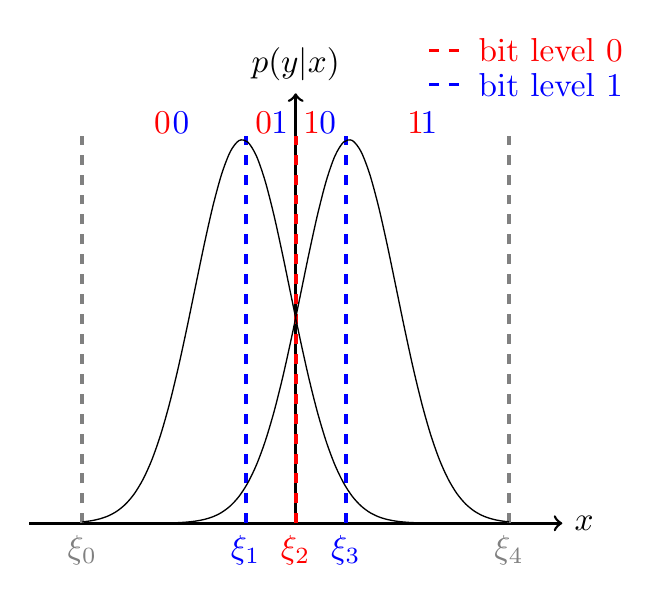
\begin{tikzpicture}[scale = 1.2]
    \begin{axis}[every axis plot post/.append style={
      mark=none,domain=-4:4,samples=50,smooth},
    clip=false,
    axis y line=none,
    axis x line*=bottom,
    ymin=0,
    xtick=\empty,
    ]
    %\draw[help lines, color=gray!30, dashed] (-4.9,0) grid (4.9,0.5);
    \draw[->, thick] (-5,0)--(5,0) node[right]{$x$};
    \draw[->, thick] (0,0)--(0,0.5) node[above]{$p(y|x)$};
    \draw[very thick, dashed, color = red] (0,0)--(0,0.45);
    \node [below, color = red] at (0,0) {{$\xi_2$}};
    \draw[very thick, dashed, color = blue] (0.9400,0)--(0.9400,0.45);
    \node [below, color = blue] at (0.9400,0) {{$\xi_3$}};
    \draw[very thick, dashed, color = blue] (-0.9400,0)--(-0.9400,0.45);
    \node [below, color = blue] at (-0.9400,0) {{$\xi_1$}};
    \draw[very thick, dashed, color = gray] (4,0)--(4,0.45);
    \node [below, color = gray] at (4,0) {{$\xi_4$}};
    \draw[very thick, dashed, color = gray] (-4,0)--(-4,0.45);
    \node [below, color = gray] at (-4,0) {{$\xi_0$}};
    \addplot [color=black] {\gauss{1}{0.8944}};
    \addplot [color=black] {\gauss{-1}{0.8944}};
    \draw[ thick, dashed, color = red ] (2.5,0.55)--(3.2,0.55) node[right]{bit level 0};
    \draw[ thick, dashed, color = blue ] (2.5,0.51)--(3.2,0.51) node[right]{bit level 1};
    \node [above, color = red] at (-2.5,0.44) {0};
    \node [above, color = blue] at (-2.15,0.44) {0};
    \node [above, color = red] at (-0.6,0.44) {0};
    \node [above, color = blue] at (-0.30,0.44) {1};
    
    
    \node [above, color = blue] at (2.5,0.44) {1};
    \node [above, color = red] at (2.25,0.44) {1};
    \node [above, color = blue] at (0.6,0.44) {0};
    \node [above, color = red] at (0.30,0.44) {1};
    
    \end{axis}
    \end{tikzpicture}
	\caption{Given the conditional probability $p(y|x)$ of symmetric BI-AWGN channel, HDQ sequentially quantizing A/D output $w$ into a 2-bit message by first finding the index $\xi_2$, then the indices $\xi_1$ and $\xi_3$.}
	\label{fig: HDQ}
\end{figure}

HDQ quantizes the symmetric BI-AWGN channel output using a  progressive \cite{nathan-hdq} or greedy approach.  
The general $b$-bit HDQ approach is as follows:
\begin{enumerate}
    \item We assume an initial high-precision uniform quantizer.  For this case, set the extreme index thresholds  $\xi_0=0$ and $\xi_{2^b}=B-1$, which are the minimum and maximum outputs of the uniform quantization.  
    \item The index threshold $\xi_{2^{(b-1)}}$ is selected as follows to determine the bit level 0:
    \begin {align}
    \xi_{2^{(b-1)}} = \arg \max_{\xi_0<\xi<\xi_{2^b}} I(X;D_1)\, , 
    \end{align}
where 
\begin{equation} 
D_1 = \mathbbm{1}(W\geq \xi_2^{(b-1)}).
% D_1 = \begin{cases} 
% 0, & \text{if } W < \xi_{2^{(b-1)}}\\
% 1, & \text{otherwise}
%\end{cases}.
\end{equation}

\item The index thresholds  $\xi_{2^{(b-2)}}$ and $\xi_{3*2^{(b-2)}}$ are selected as follows to determine bit level 1:
    \begin {align}
    \xi_{2^{(b-2)}} &= \arg \max_{\xi_0<\xi<\xi_{2^{b-1}}} I(X;D_2| D_1=0), \\ 
    \xi_{3*2^{(b-2)}} &= \arg \max_{\xi_{2^{b-1}}<\xi<\xi_{2^b}} I(X;D_2| D_1=1)\, ,
    \end{align}
    and 
\begin{equation} 
D_2 = \begin{cases} 
\mathbbm{1}(W \geq \xi_{2^{(b-2)}}) & \text{if } D_1=0 \\
\mathbbm{1}(W \geq \xi_{3*2^{(b-2)}}) & \text{if } D_1=1 \\
\end{cases}.
\end{equation}

\item In the general case, when the thresholds for $k$ previous quantization bits have been determined, $2^k$ thresholds $\{\xi_{(j+0.5)2^{b-k}}, j=0,..,2^{k}-1\}$ must be selected to determine the next quantization bit.  Each threshold maximizes $I(X;D_{k+1}|D_k=d_k, \ldots,D_1=d_1 )$ for a specific result for the $k$ previous quantization bits. 
\end{enumerate}


\begin{algorithm}[t]
    \label{alg: HDQ}
    \SetKwInOut{Input}{input}\SetKwInOut{Output}{output}\SetKwProg{Init}{initialization:}{}{}
    
    \Input{$P\left(X,W\right), X\in\{0,1\}, W\in\{0,...,B-1\}$; $b$}
    \Output{ $\{\xi_0,\xi_1,...,\xi_{2^b-1}\}$, $P(X,T)$}
    $\xi_0\leftarrow 0$, 
    $\xi_{2^b}\leftarrow B-1$\\
    \For{$i\gets0$ \KwTo $b-1$ }{
        \For{$j\gets0$ \KwTo $2^{i}-1$ }{
        $\xi_{(j+0.5)2^{b-i}} = \texttt{GSS}(\xi_{j2^{b-i}},\xi_{(j+1)2^{b-i}})$
        }
        }
    $P_{XT}(x,t)=\sum_{w=\xi_t}^{\xi_t+1}P_{XW}(x,w)$, $X\in\{0,1\}$, $T\in\{0,...,2^{b-1}\}$
    \caption{Hierarchical Dynamic Quantization }
    \end{algorithm}
Fig. \ref{fig: HDQ} illustrates how HDQ quantizes the symmetric binary input AWGN for the case where $b=2$. First, the indices  $\xi_0$  and $\xi_4$ of the extreme points are set.  Then the index $\xi_2$ is set to maximize $I(X;D_1)$.  Finally, the indices $\xi_1$ and $\xi_3$ are set to maximize $I(X;D_2| D_1)$ by independently selecting $\xi_1$ to maximize $I(X;D_2| D_1=0)$ and $\xi_3$ to maximize $I(X;D_2| D_1=1)$.


Alg. \ref{alg: HDQ} provides a full description of HDQ algorithm. The function \texttt{GSS}$(\xi_{\ell},\xi_r)$ uses the golden section search algorithm described in Sec. \ref{Sec: GSS} for thresholds search.

\bibliographystyle{uclathes}
%\bibliographystyle{thesis}
\bibliography{bio.bib}    % bibliography references

\end {document}

